\section{Solar Reflection from Shading Surfaces}\label{solar-reflection-from-shading-surfaces}

Exterior shading surfaces modeled using ``FullInteriorAndExteriorWithReflections'' can show some sky diffuse solar getting through the shades. When ``*WithReflections'' is active a partially sunlit shading surface reflects uniformly from the entire surface. If using WithReflections, shading surfaces should be broken into multiple surfaces at lines of intersection with other shading surfaces. This also includes places where another surface may tee into a shading surface.

For example, a building is shaded by surfaces A, B, and C. Shading Surface A intercepts with Shading Surfaces B and C, and are broken into three areas A1, A2, and A3. Surface A should be entered as the shown three shading areas in order to correctly model sky diffuse solar reflection from Shading Surface A.

\begin{figure}[hbtp] % fig 6
\centering
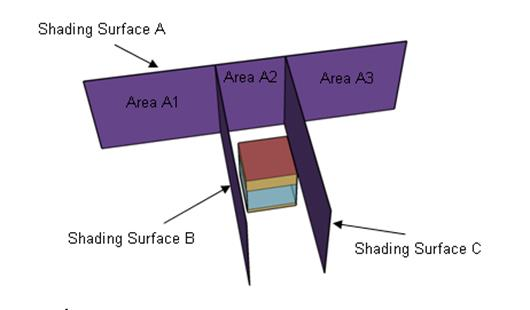
\includegraphics[width=0.9\textwidth, height=0.9\textheight, keepaspectratio=true]{media/image006.jpg}
\caption{Limitations in modeling reflections from surfaces \protect \label{fig:limitations-in-modeling-reflections-from}}
\end{figure}
